%--------------------------------------------%
% Template Beamer para Apresentações da UFRN %
% by alcemygvseverino@gmail.com              %
% Baseado em MIT Beamer Template			 %
% versao 1.1								 %
% Atualizado em 14/05/2016					 %
%--------------------------------------------%
\documentclass[]{beamer}

\mode<presentation>
{
% Para definir o tema do slide
\usetheme{Berlin}
% Para difinir cores e background
\usecolortheme{ufrn}
% Para numerar as figuras
\setbeamertemplate{caption}[numbered]
	\setbeamercovered{transparent}
}

% Para alterar a linguagem do documento
\usepackage[spanish]{babel}
% Para aceitar caracteres especias deretamente do teclado
\usepackage[utf8]{inputenc}
% Para seguir as normas da ABNT de citacao e referencias
\usepackage[alf]{abntex2cite}
% Para incluir figuras
\usepackage{graphicx}
% Para melhor ajuste da posisao das figuras
\usepackage{float}
% Para ajustar as dimensoes do layout da pagina
\usepackage{geometry}
% Para formatar estrutura e informacoes de formulas matematicas
\usepackage{amsmath}
% Para incluir simbolos especiais em formulas matematicas
\usepackage{amssymb}
% Para incluir links nas referencias
\usepackage{url}
% Para incluir paginas de documentos .pdf externos
\usepackage{pgfpages}
% Para ajustar o estilo dos contadores
\usepackage{enumerate}
% Para modificar a cor do texto
\usepackage{color}
% Para incluir condicoes
\usepackage{ifthen}
% Para colocar legendas em algo que nao e float
\usepackage{capt-of}
\usepackage{hyperref}
\usepackage{algorithm,algorithmic}
\usepackage{colortbl}

%\usepackage[T1]{fontenc}
\usepackage{inconsolata}
\usepackage{listings}

\lstset{language=Java,
basicstyle=\footnotesize\tt,        % the size of the fonts that are used for the code
 breakatwhitespace=false,         % sets if automatic breaks should only happen at whitespace
 breaklines=true,                 % sets automatic line breaking
 captionpos=b,                    % sets the caption-position to bottom
 extendedchars=true,              % lets you use non-ASCII characters; for 8-bits encodings only, does not work with UTF-8
 frame=single,                    % adds a frame around the code
 language=Java,                 % the language of the code
 keywordstyle=\bf,
 showspaces=false,                % show spaces everywhere adding particular underscores; it overrides 'showstringspaces'
 showstringspaces=false,          % underline spaces within strings only
 showtabs=false,                  % show tabs within strings adding particular underscores
 tabsize=2                       % sets default tabsize to 2 spaces
}


% Título

\title[Programaci\'on 2]{Programaci\'on 2}
\subtitle{Lenguaje Java - Manejo de Excepciones  (\emph{3era parte})\\ T\'ipos de Clases}
% Data
\date{
	\today}
% Autores
\author[Eduardo Godoy]{
	Profesor: Eduardo Godoy. \\
	\vspace{0.5mm}
	\texttt{\small eduardo.gl@gmail.com}
}
% Instituto
\institute[Universidad de Valara\'iso]{

%\texttt{\normalsize eduardo.gl@gmail.com} \\
	\vspace{0.25cm}
	\texttt Escuela de Ingenier\'ia Civil Inform\'atica.\\
	\texttt Universidad de Valpara\'iso.
}
% Logo do canto inferior direito



\begin{document}

% Sumário
\frame{\titlepage}
\section[]{}
\begin{frame}{Contenido}
	\tableofcontents
\end{frame}

% excepciones
\section{Manejo de Excepciones}
\begin{frame}{Manejo de Excepciones}
\begin{itemize}
	\item El termino Excepci\'on significa Condici\'on Excelcional dentro un programa.
	\item En java muchos evento requieren de manejo de Excepciones, Ejemplo:
	\begin{itemize}
			\item Fallas en la comunicaci\'on con componentes de Hardware.
			\item Operaciones con fuentes de almacenamiento persistente.
			\item Operaciones aritm\'eticas no permitidas.
			\item etc.
	\end{itemize}
\end{itemize}
\end{frame}

\begin{frame}{Manejo de Excepciones: ¿Como Opera?}
\begin{itemize}
	\item El manejo de Excepciones opera transfiriendo el control del programa a cierta regi\'on del programa, siempre
	dentro del mismo m\'etodo.
\end{itemize}
\begin{block}{Ejemplo.}
	Si en la ejecuci\'on de un programa se encuentra una operaci\'on de divisi\'on por 0, la ejecuci\'on del m\'etodo no continua. Luego
	se pasa a ejecutar el c\'odigo que ha sido prpeparado para manejar dicha excepci\'on.
	\end{block}
\end{frame}

\begin{frame}{Manejo de Excepciones: try - catch}
\begin{itemize}
	\item Palabra reservada \textbf{Try} es usada para definir e identificar a un segmento de c\'odigo en el cual puede ocurrir la excepci\'on.
	\item Este bloque de c\'odigo es llamado zona segura, debido a que ah\'i hay una o mas lineas riesgosas.
	\item Dentro de \textbf{catch} se indica el bloque de c\'odigo que se encargara de controlar la excepci\'on, Ejemplo:
\end{itemize}
\end{frame}

\begin{frame}{Manejo de Excepciones - try, catch}
	\begin{block}{Ejemplo.}
\lstinputlisting[language=Java,caption={},numbers=none]{resources/excepciones/EjExcepcion.java}
\end{block}
\end{frame}

\begin{frame}{Manejo de Excepciones: finally}
\begin{itemize}
	\item Palabra reservada \textbf{finally} es una secci\'on que se ejecuta siempre que independiente si la excepci\'on ocurra o no.
	\item Debido a que al ocurrir una excepci\'on esta  interrumpe la ejecuci\'on natural del c\'odigo.  Su principal funci\'on es mantener la consistencia y ejecuci\'on limpia del programa.
\end{itemize}
\end{frame}

\begin{frame}{Manejo de Excepciones - try, catch, finally}
	\begin{block}{Ejemplo.}
\lstinputlisting[language=Java,caption={},numbers=none]{resources/excepciones/Finally.java}
\end{block}
\end{frame}

\begin{frame}{Manejo de Excepciones: Declaraci\'on en m\'etodos.}
\begin{itemize}
	\item Una excepci\'on puede ser declarada en el m\'etodo, con esto se deja la responsabilidad de
	controlar la excepcion a la clase que contiene al m\'etodo que ha enviado el mensaje.
\end{itemize}
\end{frame}

\begin{frame}{Manejo de Excepciones - Declaraci\'on en m\'etodos}
	\begin{block}{Ejemplo.}
\lstinputlisting[language=Java,caption={},numbers=none]{resources/excepciones/TryCatchDecl.java}
\end{block}
\end{frame}

\begin{frame}{Manejo de Excepciones - Declaraci\'on en m\'etodos}
	\begin{block}{Ejemplo.}
\lstinputlisting[language=Java,caption={},numbers=none]{resources/excepciones/TryCatchDecl0.java}
\end{block}
\end{frame}


% Wrappers
\section{Wrapper  class}
\begin{frame}{Final  class}
\begin{block}{Consideraciones}
\begin{itemize}{}
\item Proveer un mecanismo para cubrir un valor primitivo con caracter\'isticas de objetos.
\item En Java existe una clase Wrapper para todo dato primitivo.
\end{itemize}
\end{block}
\end{frame}

\begin{frame}{Final  class}
\begin{block}{Alugunos Wrappers}
	\begin{center}
	\begin{tabular}{ | c c c | }
		\hline
		primitive & Wrapper class & Constructor Args.\\
		\hline
	 boolean & Boolean & boolean o String \\
	 \hline
	 byte & Byte &  byte o String \\
	 \hline
	 char & Char & char   \\
	 \hline
	 double & Double & double o String \\
	 \hline
	 float & Float & float, double o  String \\
	 \hline
	 int  & Integer & int o String \\
	 \hline
	 long & Long & log  Strin \\
	 \hline
	 short & Short & ceshort o String\\
	 \hline
	\end{tabular}
	\end{center}
\end{block}
\end{frame}



\begin{frame}{Manejo de Excepciones - Declaraci\'on en m\'etodos}
	\begin{block}{Ejemplo.}
\lstinputlisting[language=Java,caption={},numbers=none]{resources/excepciones/Wrappers.java}
\end{block}
\end{frame}
 

% apislib
\section{API}
\begin{frame}{API}
\begin{itemize}{}
\item \textbf{API} - \textit{Application Programming Interface}.
\item Es un conjunto de clases y m\'etodos que permiten comunicarse con otras otros programas, componentes o servicios.
\item La \textbf{API de Java} provee las funcionalidades necesarias para permitirnos utilizar sus caracter\'isticas o ventajas sobre los otros lenguajes.
\item Java cuenta con APIS para diversos objetivos, como por ejemplo, conectarse a un componente de Hardware, servicios en internet (sistemas de pago online), Comunicarse con tros lenguajes de programaci\'on, bases de datos, lenguajes de etiquetado (XML), etc.
\end{itemize}
\end{frame}

\begin{frame}{API}

\begin{block}{En general}
  Se conoce como API en java a un conjunto de librerias cuyos \textbf{imports} en nuestros programas nos ayudan a solucionar un problema de integraci\'on o comunicaci\'on espec\'ifico
\end{block}

\end{frame}


\begin{frame}{API - Ejemplo.}
  \begin{figure}
    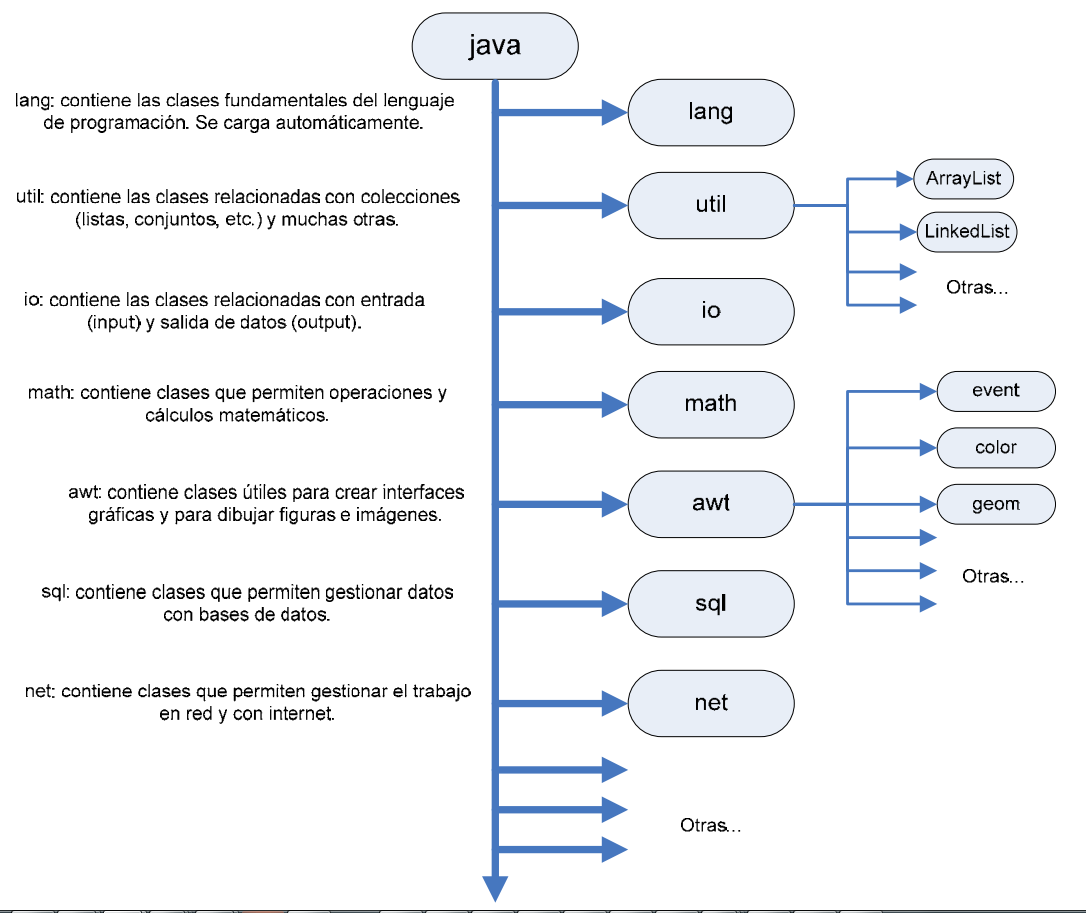
\includegraphics[scale=0.3]{figuras/API_Java.PNG}
  \end{figure}
\end{frame}

\begin{frame}{API - Ejemplo.}
  \begin{figure}
    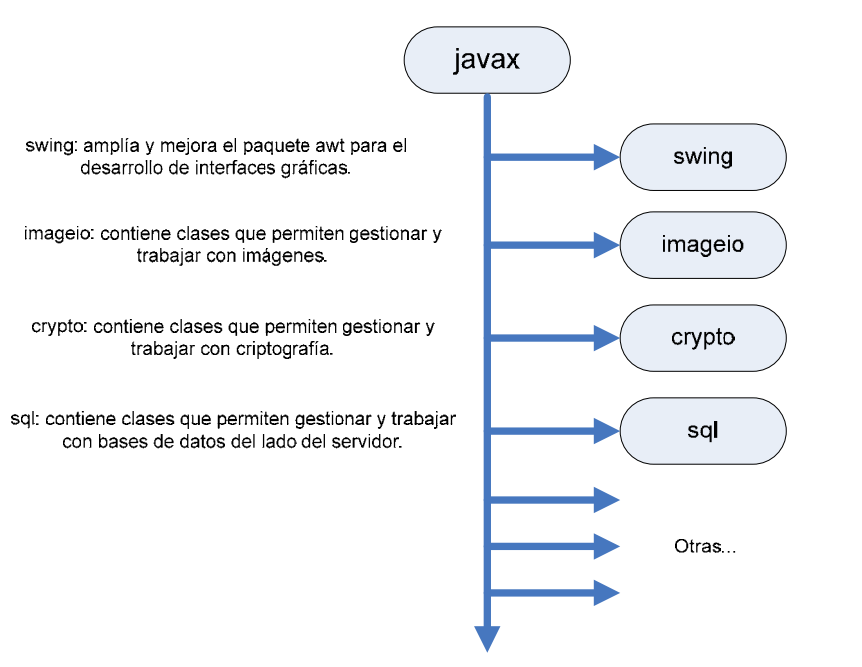
\includegraphics[scale=0.4]{figuras/API_Javax.PNG}
  \end{figure}
\end{frame}

\begin{frame}{Manejo de Excepciones - Declaraci\'on en m\'etodos}
	\begin{block}{Ejemplo.}
\lstinputlisting[language=Java,caption={},numbers=none]{resources/apis/Imports.java}
\end{block}
\end{frame}


% tips
\section{TIPs}

\begin{frame}{Tips - Ocultamiento de Informaci\'on - Ejemplo.}
  \begin{figure}
    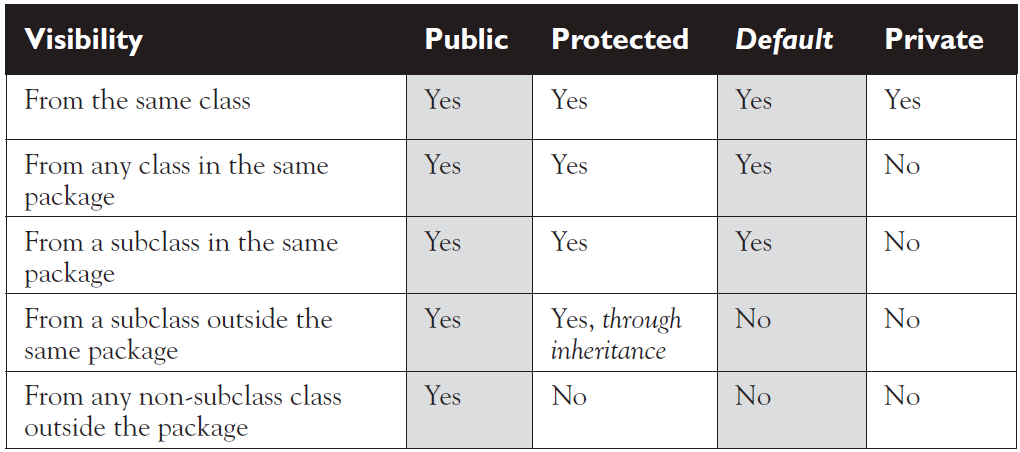
\includegraphics[scale=0.4]{figuras/ocultamiento_tabla.PNG}
  \end{figure}
\end{frame}

\begin{frame}{Tips - Casting}
	\begin{block}{Ejemplo.}
\lstinputlisting[language=Java,caption={},numbers=none]{resources/tips/Animal.java}
\end{block}
\end{frame}

\begin{frame}{Tips - Casting}
	\begin{block}{Ejemplo.}
\lstinputlisting[language=Java,caption={},numbers=none]{resources/tips/MainAnimal.java}
\end{block}
\end{frame}


% Referencias
%\section{Referencias}
\begin{frame}{Referências}
	Suas referencias bibliográficas aqui, siga o modelo ABNT.
	\bibliography{bib/bibliografia}
\end{frame}

% Agradecimentos
\section{}
%\begin{frame}{Agradecimentos}
%	Agradeço a todos.
%\end{frame}

\end{document}
